%%%%%%%%%%%%%%%%%%%%%%%%%%%%%%%%%%%%%%%%%%%%%%%%%%%%%%%%%%%%%%%%%%%%%%%
\documentclass
  [ 12pt
  %twoside            % beidseitiger Druck
  , openright          % Kapitel beginnen auf einer rechten Seite
  , listof=totoc       % Verzeichnisse im Inhaltsverzeichnis
  , bibliography=totoc % Literaturverzeichnis im Inhaltsverzeichnis
  , parskip=full       % Absätze durch einen vergrößerten Zeilenabstand getrennt
%  , draft              % Entwurfsversion
  ]{scrreprt}          % Dokumentenklasse: KOMA-Script Buch

%%%%%%%%%%%%%%%%%%%  Document info  %%%%%%%%%%%%%%%%%%%%%%%%%%%%%%%
\newcommand{\projname}{Bachelor Thesis}
\newcommand{\titel}{Analyse der Zeitersparnis der Verwendung eines Templates bei der Erstellung einer Bachelor Thesis}
\newcommand{\untertitel}{}
\newcommand{\thesisname}{Bachelor Thesis}
\newcommand{\Datum}{23. Februar 20XX}
\newcommand{\authorname}{Maximilian Mustermann}
%%%%%%%%%%%%%%%%%%%  Document info  %%%%%%%%%%%%%%%%%%%%%%%%%%%%%%%

%%%%%%%%%%%%%%%%%%%%%%%%%%%%%%%%%%%%%%%%%%%%%%%%%%%%%%%%%%%%%%%%%%%%%%%
% Packages
%%%%%%%%%%%%%%%%%%%%%%%%%%%%%%%%%%%%%%%%%%%%%%%%%%%%%%%%%%%%%%%%%%%%%%%
\usepackage{scrhack}
\usepackage{url}
\usepackage{wrapfig}
\usepackage{xcolor}
\usepackage[font=footnotesize]{caption}
\setlength{\abovecaptionskip}{5pt}
\setlength{\belowcaptionskip}{10pt}
\usepackage{listings}
\usepackage{makecell}
\usepackage{array}
%\usepackage{scrextend}
\newcolumntype{x}[1]{>{\centering\let\newline\\\arraybackslash\hspace{0pt}}p{#1}}
\newcommand{\paragraphnl}[1]{\paragraph{#1}\mbox{}\\\vspace{-1cm}}

\newcommand{\tabitem}{~~\llap{\textbullet}~~}

\usepackage{ifpdf}
\ifpdf
  \usepackage{ae}               % Fonts für pdfLaTeX, falls keine cm-super-Fonts installiert
  \usepackage{microtype}        % optischer Randausgleich, falls pdflatex verwandt
  \usepackage[pdftex]{graphicx} % Grafiken in pdfLaTeX
\else
  \usepackage[dvips]{graphicx}  % Grafiken und normales LaTeX
\fi

\usepackage[a4paper,%
    %bindingoffset=0.5cm,%
    left=3.5cm,
    right=3.0cm,
    top=3.0cm,
    bottom=3.0cm,
    footskip=1.0cm,
    includeheadfoot
]{geometry}
            
\usepackage[utf8]{inputenc}         % Input encoding (allow direct use of special characters like "ä")
%\usepackage[english]{babel}
\usepackage[ngerman]{babel}
\usepackage[T1]{fontenc}
\usepackage[printonlyused]{acronym} % list of acronyms and abbreviations
\usepackage[automark]{scrlayer-scrpage} 	 % Schickerer Satzspiegel mit KOMA-Script
\usepackage{setspace}           	 % Allow the modification of the space between lines
\usepackage{booktabs}           	 % Netteres Tabellenlayout
\usepackage{multicol}               % Mehrspaltige Bereiche
\usepackage{multirow}
\usepackage{quotchap}               % Beautiful chapter decoration
\usepackage{subfig}                 % allow sub figures
\usepackage{tabularx}               % Tabellen mit fester Breite
\usepackage{longtable}
\usepackage[
    backend=biber,
    style=numeric,
    natbib=true,
    sorting=nty 
]{biblatex}
\addbibresource{sources.bib}
% COdeblock stuff
\usepackage{listings}
\usepackage{csquotes}

\ifpdf
  \usepackage{hyperref}
  \definecolor{darkblue}{rgb}{0,0,.5}
  \hypersetup
  	{ colorlinks=true
  	, breaklinks=true
    , linkcolor=black
    , menucolor=black
    , urlcolor=black
    , citecolor=black
    , pdftitle={\projname -- \untertitel}
    , pdfsubject={\thesisname}
    , pdfauthor={\authorname}
    }
\else
\fi


%%%%%%%%%%%%%%%%%%%%%%%% Listings (Code Blocks) %%%%%%%%%%%%%%%%%%%%%%%%%%%%%%%%%%%

\usepackage{listings}
\KOMAoptions{listof=totoc} % necessary because of scrhack
\renewcommand{\lstlistlistingname}{List of Listings}
\lstset
  { basicstyle=\small\ttfamily
  , breaklines=false
  , captionpos=b
  , showstringspaces=false
  , keywordstyle={}
  }

\renewcommand{\lstlistlistingname}{Quelltextverzeichnis}
\renewcommand{\lstlistingname}{Quelltext}


\definecolor{codegreen}{rgb}{0.22, 0.85, 0.35}
\definecolor{codeblue}{rgb}{0.22, 0.51, 0.85}
\definecolor{codeyellow}{rgb}{0.61, 0.55, 0.04}
\definecolor{codeorange}{rgb}{0.85, 0.69, 0.22}
\definecolor{codegray}{rgb}{0.5,0.5,0.5}
\definecolor{codepurple}{rgb}{0.58,0,0.82}
\definecolor{codered}{rgb}{0.85, 0.22, 0.27}
\definecolor{backcolour}{rgb}{0.95,0.95,0.92}

\definecolor{numbercolor}{rgb}{0.7,0.43,0}

\lstdefinelanguage{sql}{
    morekeywords={
        ADD, CONSTRAINT, ALTER, COLUMN, TABLE, ALL, AND, ANY, AS, ASC, BACKUP, DATABASE, BETWEEN, CASE, CHECK, COLUMN, CREATE, INDEX, REPLACE, VIEW, PROCEDURE, UNIQUE, DEFAULT, DELETE, DESC, DISTINCT, DROP, EXEC, EXISTS, FOREIGN, KEY, FROM, FULL, OUTER, JOIN, GROUP, BY, HAVING, IN,  INNER, INSERT, INTO, IS, NULL, NOT, LEFT, LIKE, LIMIT, OR, ORDER, PRIMARY, RIGHT, ROWNUM, SELECT, TOP, SET, TRUNCATE, UNION, UPDATE, VALUES, WHERE, RETURNING, RETURNS, LANGUAGE, SQL, COALESCE, WHEN, THEN, BEGIN, END, ON, LEAKPROOF, DECLARE, NEW, IF, RAISE, EXCEPTION, RETURN, FUNCTION, OWNER, TO, ELSE, BEFORE, FOR, EACH, ROW, EXECUTE, INCLUDE, USING, integer, int, IF, ELSIF, NULLS, FIRST, TRIGGER
    },
    backgroundcolor=\color{white},
    commentstyle=\color{codegreen},
    keywordstyle=\color{codered},
    stringstyle=\color{codegreen},
    basicstyle=\ttfamily\linespread{1}\footnotesize,
    morecomment=[l]{--},
    breakatwhitespace=true,
    breaklines=false,
    morestring=[b][\color{codegreen}]{'},
    morestring=[b][\color{codeblue}]{"},
    captionpos=b,
    keepspaces=true,
    showspaces=false,
    showstringspaces=false,
    showtabs=false,
    tabsize=2,
    showlines=true,
    literate=
        *{0}{{{\color{numbercolor}0}}}{1}
         {1}{{{\color{numbercolor}1}}}{1}
         {2}{{{\color{numbercolor}2}}}{1}
         {3}{{{\color{numbercolor}3}}}{1}
         {4}{{{\color{numbercolor}4}}}{1}
         {5}{{{\color{numbercolor}5}}}{1}
         {6}{{{\color{numbercolor}6}}}{1}
         {7}{{{\color{numbercolor}7}}}{1}
         {8}{{{\color{numbercolor}8}}}{1}
         {9}{{{\color{numbercolor}9}}}{1}
        {Ö}{{\"O}}1
        {Ä}{{\"A}}1
        {Ü}{{\"U}}1
        {ß}{{\ss}}1
        {ü}{{\"u}}1
        {ä}{{\"a}}1
        {ö}{{\"o}}1
        {\ \ }{{\ }}1
}

\lstdefinelanguage{sql_no_num}{
    morekeywords={
        ADD, CONSTRAINT, ALTER, COLUMN, TABLE, ALL, AND, ANY, AS, ASC, BACKUP, DATABASE, BETWEEN, CASE, CHECK, COLUMN, CREATE, INDEX, REPLACE, VIEW, PROCEDURE, UNIQUE, DEFAULT, DELETE, DESC, DISTINCT, DROP, EXEC, EXISTS, FOREIGN, KEY, FROM, FULL, OUTER, JOIN, GROUP, BY, HAVING, IN,  INNER, INSERT, INTO, IS, NULL, NOT, LEFT, LIKE, LIMIT, OR, ORDER, PRIMARY, RIGHT, ROWNUM, SELECT, TOP, SET, TRUNCATE, UNION, UPDATE, VALUES, WHERE, RETURNING, RETURNS, LANGUAGE, SQL, COALESCE, WHEN, THEN, BEGIN, END, ON, LEAKPROOF, DECLARE, NEW, IF, RAISE, EXCEPTION, RETURN, FUNCTION, OWNER, TO, ELSE, BEFORE, FOR, EACH, ROW, EXECUTE, INCLUDE, USING, integer, int, IF, ELSIF, NULLS, FIRST, TRIGGER
    },
    backgroundcolor=\color{white},
    commentstyle=\color{codegreen},
    keywordstyle=\color{codered},
    stringstyle=\color{codegreen},
    basicstyle=\ttfamily\linespread{1}\footnotesize,
    morecomment=[l]{--},
    morestring=[b]{'},
    breakatwhitespace=true,
    breaklines=false,
    captionpos=b,
    keepspaces=true,
    showspaces=false,
    showstringspaces=false,
    showtabs=false,
    tabsize=2,
    showlines=true,
    literate=
        {Ö}{{\"O}}1
        {Ä}{{\"A}}1
        {Ü}{{\"U}}1
        {ß}{{\ss}}1
        {ü}{{\"u}}1
        {ä}{{\"a}}1
        {ö}{{\"o}}1
        {\ \ }{{\ }}1
}

\usepackage{bera}
\definecolor{eclipseStrings}{RGB}{42,0.0,255}
\definecolor{eclipseKeywords}{RGB}{127,0,85}
\colorlet{numb}{magenta!60!black}

\lstdefinelanguage{json}{
    basicstyle=\ttfamily\linespread{1}\footnotesize,
    commentstyle=\color{black},
    stringstyle=\color{codegreen},
    numbers=left,
    numberstyle=\color{black},
    xleftmargin=1.5em,
    stepnumber=1,
    numbersep=8pt,
    tabsize=2,
    showstringspaces=false,
    breaklines=false,
    frame=lines,
%    backgroundcolor=\color{gray}, %only if you like
    morestring=[b]",
    morestring=[d]]’,
%    comment=[l]{:\ "},
%    morecomment=[l]{:"},
    keywordstyle=\color{numb},
    literate=
        *{0}{{{\color{numbercolor}0}}}{1}
         {1}{{{\color{numbercolor}1}}}{1}
         {2}{{{\color{numbercolor}2}}}{1}
         {3}{{{\color{numbercolor}3}}}{1}
         {4}{{{\color{numbercolor}4}}}{1}
         {5}{{{\color{numbercolor}5}}}{1}
         {6}{{{\color{numbercolor}6}}}{1}
         {7}{{{\color{numbercolor}7}}}{1}
         {8}{{{\color{numbercolor}8}}}{1}
         {9}{{{\color{numbercolor}9}}}{1}
         {null}{{{\color{numbercolor}null}}}{4}
         {true}{{{\color{numbercolor}true}}}{5}
         {false}{{{\color{numbercolor}false}}}{5}
        {Ö}{{\"O}}1
        {Ä}{{\"A}}1
        {Ü}{{\"U}}1
        {ß}{{\ss}}1
        {ü}{{\"u}}1
        {ä}{{\"a}}1
        {ö}{{\"o}}1
        {\ \ }{{\ }}1
}

\lstdefinestyle{annotation_style}{
    morestring=[s][\color{black}]{"atn_id}{":},
    morestring=[s][\color{black}]{"timestamp}{":},
    morestring=[s][\color{black}]{"annotation}{":},
    morestring=[s][\color{black}]{"valid_from}{":},
    morestring=[s][\color{black}]{"valid_until}{":}
}

\lstdefinelanguage{python}{
    morekeywords=[1]{
        None,and,as,assert,break,class,continue,def,del,elif,
        else,except,finally,for,from,global,if,import,in,is,lambda,nonlocal,
        not,or,pass,print,raise,return,try,while,with,yield,repeat,
        Exception,False,True,abs,all,any,ascii,bin,bool,bytearray,
        bytes,callable,chr,classmethod,compile,complex,copyright,delattr,dict,
        dir,divmod,enumerate,eval,exec,exit,float,format,frozenset,getattr,
        globals,hasattr,hash,help,hex,id,input,int,isinstance,issubclass,iter,
        len,license,list,locals,map,max,min,next,object,oct,open,ord,pow,
        property,quit,range,repr,reversed,round,set,setattr,slice,sorted,
        staticmethod,str,sum,super,tuple,type,vars,zip,inputInt,inputFloat,
        inputString,msgDlg,askYesNo,enum,clrScr,head,tail,indices,self
    },
    keywordstyle=[1]\color{codered},
    morekeywords=[2]{
        Database, Cursor,
        Enum, BaseModel, Extra, StrictInt, Coordinate, BoundingBox, Orientation, Eyes, Gender, AnnotationBase, AnnotationAllowExtra, AnnotationForbidExtra
    },
    keywordstyle=[2]\color{codeyellow},
    basicstyle=\ttfamily\linespread{1}\footnotesize, % \ttfamily\small  \normalfont\ttfamily
    commentstyle=\color{eclipseStrings},
    stringstyle=\color{codegreen},
    xleftmargin=1.5em,
    tabsize=2,
    numbers=left,
    numberstyle=\color{black},
    stepnumber=1,
    numbersep=8pt,
    showstringspaces=false,
    breaklines=false,
    frame=lines,
    morecomment=[l]\#,
    morestring=[b]',
    morestring=[b]",
    morestring=[b]{'''},
    morestring=[b]{"""},
    literate=
        {Ö}{{\"O}}1
        {Ä}{{\"A}}1
        {Ü}{{\"U}}1
        {ß}{{\ss}}1
        {ü}{{\"u}}1
        {ä}{{\"a}}1
        {ö}{{\"o}}1
        {\ \ }{{\ }}1
}

\lstdefinelanguage{pseudo}{
    morekeywords={
        function, IF, THEN, ELSE, END, return, WHILE, FOR, NOT, IS, public, private, TRY, CATCH, EXCEPTION, RETHROW, IN, THROW, GET, WITH, EACH, RETURN
    },
    keywordstyle=\color{codered},
    basicstyle=\ttfamily\linespread{1}\footnotesize, % \ttfamily\small  \normalfont\ttfamily
    commentstyle=\color{eclipseStrings},
    stringstyle=\color{codegreen},
    xleftmargin=1.5em,
    tabsize=2,
    numbers=left,
    numberstyle=\color{black},
    stepnumber=1,
    numbersep=8pt,
    showstringspaces=false,
    breaklines=false,
    frame=lines,
    morecomment=[l]//,
    morestring=[b]',
    morestring=[b]",
    literate=
        {Ö}{{\"O}}1
        {Ä}{{\"A}}1
        {Ü}{{\"U}}1
        {ß}{{\ss}}1
        {ü}{{\"u}}1
        {ä}{{\"a}}1
        {ö}{{\"o}}1
        {\ \ }{{\ }}1
}

\lstset{aboveskip=0.25cm,belowskip=0pt}

\renewcommand\theadfont{}

\begin{document}

\pagenumbering{Roman}

%%%%%%%%%%%%%%%%%%%%%%%%%%%%%%%%%%%%%%%%%%%%%%%%%%%%%%%%%%%%%%%%%%%

% Titelseite
\newgeometry{left=3cm,right=2cm,top=2.0cm,bottom=2.0cm}

\titlehead{
    \centering
    
\includegraphics[width=.5\textwidth]{bilder/fhw}\\
    \bigskip
    \textsc{\Large Department of Computer Science}
}

\subject{\Large \thesisname}
\title{\Large \titel}
\subtitle{\large \untertitel}
\date{
    \vspace{-1cm}
    {\small Abgabedatum:}\\
    \medskip
    \Datum
}
\author{}
\publishers{

\vfill
\normalsize
    
\raggedright
{\small Eingereicht von:} \\
\smallskip
{\Large \authorname}\\
Musterstraße 5a\\
22880 Wedel\\
Tel.: 01234 56789\\
E-Mail: inf123456@stud.fh-wedel.de\\

\bigskip
\bigskip

\begin{minipage}{0.48\linewidth}
\raggedright
    {\small Referent:}\\
    \smallskip
    {\Large Prof. Dr. Vorname Nachname}\\
    Fachhochschule Wedel\\
    Feldstraße 143\\
    22880 Wedel\\
    Telefon: 04103 - 8048 - XX\\
    E-Mail: xx@fh-wedel.de
\end{minipage}
\begin{minipage}{0.5\linewidth}
\raggedleft
    {\small Betreut von:}\\
    \smallskip
    {\Large Vorname M. Nachname}\\
    Ein FIRMA GmbH\\
    Firmenweg 50\\
    20148 Hamburg\\
    Telefon: 01234 56789\\
    E-Mail: vorname.nachname@firma.com
\end{minipage}
    
}

\maketitle


\restoregeometry

%%%%%%%%%%%%%%%%%%%%%%%%%%%%%%%%%%%%%%%%%%%%%%%%%%%%%%%%%%%%%%%%%%%

% Mehr Platz für Nummerierung benötigt in Verzeichnissen, wenn ein Kapitel 10 oder mehr Bilder hat
\DeclareTOCStyleEntry[numwidth=3em]{tocline}{figure} % Für Abbildungsverzeichnis
%\DeclareTOCStyleEntry[numwidth=3em]{tocline}{table} % Für Tabellenverzeichnis

\tableofcontents
\listoffigures
\listoftables
\cleardoublepage

%%%%%%%%%%%%%%%%%%%%%%%%%%%%%%%%%%%%%%%%%%%%%%%%%%%%%%%%%%%%%%%%%%%

\pagenumbering{arabic}

\begin{onehalfspace}

\begin{abstract}
\paragraphnl{Abstract}

{\small
Hier kommt gegebenenfalls ein Abstract hin, welches kurz die gesamte Arbeit inkl. dem Ergebnis zusammenfasst.

 Lorem ipsum dolor sit amet, consectetur adipiscing elit. Cras quis facilisis dui. Fusce pulvinar sagittis nibh vitae vehicula. Duis pulvinar egestas lacus non varius. Phasellus interdum interdum lectus, quis euismod neque viverra a. Aliquam erat volutpat. In felis felis, semper in ullamcorper vitae, commodo sed ipsum. Cras consequat lorem nibh. Duis vulputate tellus ante, eu porttitor tellus tempor ac. Praesent eget nisl condimentum, rhoncus magna sit amet, luctus ipsum. Nunc vestibulum condimentum turpis, ac finibus odio consectetur eu. Ut volutpat risus non sapien dignissim efficitur. Sed scelerisque metus at posuere condimentum. Vivamus finibus, neque et cursus malesuada, orci purus scelerisque arcu, ut sollicitudin neque mi eu massa. Pellentesque at luctus ipsum. Praesent eu hendrerit est. Sed blandit sem sem, vel condimentum lectus fermentum consectetur.

Sed quis sem vitae enim molestie dapibus. Sed sodales nulla luctus tristique porttitor. Nullam sit amet semper risus. Fusce mi purus, blandit vel felis et, placerat ultricies urna. Mauris pretium mi ac felis lacinia porta. Class aptent taciti sociosqu ad litora torquent per conubia nostra, per inceptos himenaeos. Curabitur sit amet turpis eget enim iaculis sollicitudin non non libero. Vestibulum auctor dictum sapien, vitae rutrum mauris. Aenean fringilla neque non risus vestibulum, a bibendum leo tempus. Nunc consectetur posuere neque non rutrum. Nullam volutpat mauris et ex pretium aliquam. 
}
\end{abstract}
\chapter{Einleitung}

Einleitung beginnt hier. 
Hier ein Beispiel eines Zitats:
\begin{quote}
According to all known laws
of aviation,

there is no way a bee
should be able to fly.

Its wings are too small to get
its fat little body off the ground.
\footnote{
Simon Smith und Steve Hickner, 
url: \url{http://www.script-o-rama.com/movie_scripts/a1/bee-movie-script-transcript-seinfeld.html}, 
Abrufdatum: 2022-02-18\cite{bee_movie}
}
\end{quote}
\vspace{-0.5cm} % negative vertical spacing
\begin{flushright}
{\footnotesize Note: Not true.} 
\end{flushright}

Anführungszeichen können durch den Befehl \textbackslash{}enquote \enquote{verwendet} werden, da es an den Sprach-Style angepasst werden kann und "das" nicht korrekt dargestellt wird.
Sonderzeichen wie z. B. Unterstriche müssen aber gesondert behandelt werden \enquote{ein\_wort}.

Beispiele für mathematische Formeln:
\begin{enumerate}
    \item $\mathbf{Q} = \{{\frac{a}{b}} \mid a,b \in \mathbf{Z} , b \neq 0\}
        \Rightarrow |\mathbf{Q}| \leq 1$
    \item $(x \neq 0 \; \land \; (y = 0 \; \lor \; x < y))$
    \item $\sim150$
\end{enumerate}

\clearpage % Page-Break

Eine nicht-nummerierte Liste:
\begin{itemize}
    % reduce spacing between items
    \setlength{\itemsep}{5pt}
    \setlength{\parskip}{0pt}
    \setlength{\parsep}{0pt}
    %
    \item The bee, of course, flies anyway
    \item because bees don't care what humans think is impossible.
    \item Yellow, black. Yellow, black. Yellow, black. Yellow, black.
    \item Ooh, black and yellow! Let's shake it up a little.
\end{itemize}


\section{Problembeschreibung}

Hier kann z.B. das Problem erläutert werden, aus welchem die Thesis entstanden ist.

Lorem ipsum dolor sit amet, consectetur adipiscing elit. Integer efficitur ipsum ut nulla dignissim tincidunt. Nullam sit amet tempor urna. Ut euismod mattis orci, vel mattis mi malesuada in. Aliquam molestie fermentum vestibulum. Cras egestas molestie ipsum, vitae malesuada ante consectetur id. In turpis neque, pharetra eget neque vel, rhoncus tincidunt ex. Sed lacinia fermentum odio quis faucibus. Phasellus blandit orci vitae ipsum rutrum aliquam. Fusce ipsum nisl, luctus in interdum non, sodales sed lacus. Fusce vitae fermentum tellus, vitae feugiat magna. Curabitur tincidunt mauris ac venenatis accumsan. Mauris efficitur sit amet mauris in sodales. Ut fringilla commodo sem, at commodo erat mattis sed.

Integer venenatis convallis erat, sit amet elementum odio egestas interdum. Phasellus sagittis vestibulum libero vel sodales. Phasellus a facilisis felis, vel mollis velit. Quisque pulvinar turpis vitae bibendum condimentum. Nulla facilisi. Praesent iaculis euismod eros et consequat. Nullam efficitur facilisis sapien. Aenean non laoreet lectus. Phasellus tellus lorem, ullamcorper vel aliquam ut, sollicitudin accumsan nibh. Duis vel elementum justo. Proin sed enim ipsum. Morbi sed mattis neque. Nulla varius dui a purus tempor elementum. Donec at nisl tortor. Pellentesque consequat porta aliquet. 

\clearpage

\begin{figure}[ht]
    \centering
    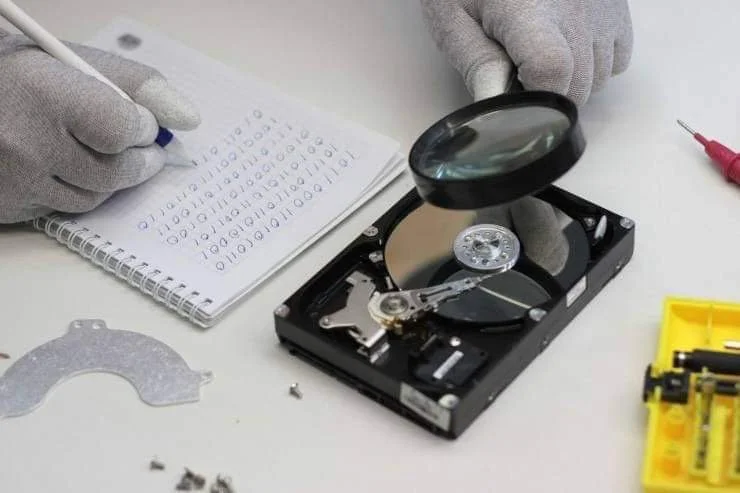
\includegraphics[width=0.8\textwidth]{bilder/read_hard_drive.png} % 80% der Textbreite
    \caption
    [Auslesen einer Festplatte] % Text, der im Bildverzeichnis verwendet wird
    {Auslesen einer Festplatte\cite{quelle}} % citation in der Beschriftung aber nicht im Bildverzeichnis
    \label{fig:old_db}
\end{figure}

\begin{wraptable}[9]{r}{8cm} 
% [9] = Höhe von neun Zeilen, {r} = rechts, {8cm} = Breite von 8cm (0.6\textwidth geht z.B. auch)
\begin{center}
\begin{tabular}{||c c c||} 
    \hline
    Name & anderer Name & eine Anzahl \\ [0.5ex] 
    \hline\hline
    Joanne &
    Esparza &
    $\sim$ 35 \\
    \hline
    Ivor &
    Sullivan &
    $\sim$ 82 \\ 
    \hline
    Martin & 
    Southern &
    $\sim$ 35 \\
    \hline
    Karina & 
    Willis &
    $\sim$ 32 \\
    \hline
\end{tabular}
\end{center}
\caption{Anzahl Einträge in den Tabellen}
\label{tab:bsp_tabelle}
\end{wraptable} 

Hier noch eine Grundlegende Tabelle, die neben dem Text steht.
Die Tabelle \ref{tab:bsp_tabelle} kann durch das Label referenziert werden.
Auf gleiche Weise können auch Kapitel, Bilder, etc. referenziert werden.

Lorem ipsum dolor sit amet, consectetur adipiscing elit. Integer efficitur ipsum ut nulla dignissim tincidunt. Nullam sit amet tempor urna. Ut euismod mattis orci, vel mattis mi malesuada in. Aliquam molestie fermentum vestibulum. 

Cras egestas molestie ipsum, vitae malesuada ante consectetur id. In turpis neque, pharetra eget neque vel, rhoncus tincidunt ex. Sed lacinia fermentum odio quis faucibus. Phasellus blandit orci vitae ipsum rutrum aliquam. Fusce ipsum nisl, luctus in interdum non, sodales sed lacus. 


\clearpage

\section{Überblick}
\label{kap:ueberblick}

Hier kann ein Überblick über folgenden Kapitel dargestellt werden.

Lorem ipsum dolor sit amet, consectetur adipiscing elit. Integer efficitur ipsum ut nulla dignissim tincidunt. Nullam sit amet tempor urna. Ut euismod mattis orci, vel mattis mi malesuada in.

In turpis neque, pharetra eget neque vel, rhoncus tincidunt ex. Sed lacinia fermentum odio quis faucibus. 

Phasellus blandit orci vitae ipsum rutrum aliquam. Fusce ipsum nisl, luctus in interdum non, sodales sed lacus. Fusce vitae fermentum tellus, vitae feugiat magna. Curabitur tincidunt mauris ac venenatis accumsan. 
\chapter{Grundlagen}

In diesem Kapitel werden die Grundlagen der verwendeten Themen und Technologien erläutert, die für das Verständnis der folgenden Arbeit notwendig sind.

% \paragraphnl ist ein custom command. Ein \paragraph plus ein line-break / new-line.
% (Nach \paragraphnl{Paragraph} muss eine Zeile frei gelassen werden.)

\section{Kapitel\#1}

Lorem ipsum dolor sit amet, consectetur adipiscing elit. Integer efficitur ipsum ut nulla dignissim tincidunt. Nullam sit amet tempor urna. Ut euismod mattis orci, vel mattis mi malesuada in. 

\section{Kapitel\#2}

Aliquam molestie fermentum vestibulum. Cras egestas molestie ipsum, vitae malesuada ante consectetur id. In turpis neque, pharetra eget neque vel, rhoncus tincidunt ex. 


\subsection{Unterkapitel\#1}

Sed lacinia fermentum odio quis faucibus. Phasellus blandit orci vitae ipsum rutrum aliquam. 

\subsection{Unterkapitel\#2}

Fusce ipsum nisl, luctus in interdum non, sodales sed lacus. 

\paragraphnl{Paragraph}

Fusce vitae fermentum tellus, vitae feugiat magna. 

\subsubsection{Unter-Unterkapitel\#1}

Curabitur tincidunt mauris ac venenatis accumsan. 

\subsubsection{Unter-Unterkapitel\#2}

Mauris efficitur sit amet mauris in sodales. 

\subsubsection{Unter-Unterkapitel\#3}

Ut fringilla commodo sem, at commodo erat mattis sed. 

\subsection{Unterkapitel\#3}

Integer aliquet orci nec ligula aliquam accumsan. 

\subsubsection{Unter-Unterkapitel\#1}

Nullam auctor rhoncus ultrices. Nunc viverra consequat interdum. 

\subsubsection{Unter-Unterkapitel\#2}

Integer venenatis convallis erat, sit amet elementum odio egestas interdum. 

\subsubsection{Unter-Unterkapitel\#3}

Phasellus sagittis vestibulum libero vel sodales. 

\section{Kapitel\#3}

Phasellus a facilisis felis, vel mollis velit. 

\subsection{Unterkapitel\#1}

Quisque pulvinar turpis vitae bibendum condimentum. 

\subsection{Unterkapitel\#2}

Nulla facilisi. Praesent iaculis euismod eros et consequat. Nullam efficitur facilisis sapien. 

\subsubsection{Unter-Unterkapitel\#1}

Aenean non laoreet lectus. Phasellus tellus lorem, ullamcorper vel aliquam ut, sollicitudin accumsan nibh. 

\subsection{Unterkapitel\#3}

Duis vel elementum justo. Proin sed enim ipsum. 

\chapter{Hauptkapitel\#1}

Dieses Kapitel konkretisiert die bereits genannten Problematiken, schildert und vergleicht mögliche Umsetzungsvarianten, um diese zu vergleichen und daraus eine Auswahl zu treffen.
Hier werden auch regelmäßig die Grundlagen referenziert.


\section{weitere Beispiele}

\begin{table}[ht]
\centering
    \begin{tabular}{l r | r}
        \hline\hline
        \thead{Tabelle}
        &
        \thead{\# Einträge}
        &
        \thead{Proz. Anteil der\\ursprünglichen Einträge} \\ [0.5ex] 
        % \thead erlaubt Zeilenumbruch in header
        % [0.5ex] = Abstand zur nächsten Zeile
        \hline
        Face Position Orientation   & $\sim$ 67.847.000 (73.3 \%) &  100.0 \%\\
        Face Demographics           & $\sim$ 24.377.000 (26.3 \%) &   36.0 \%\\
        Image Details               &    $\sim$ 161.000 ( 0.2 \%) &    0.2 \%\\
        Face Details                &    $\sim$ 144.000 ( 0.2 \%) &    0.2 \%\\
        \hline
        \textbf{Gesamt}             &        92.528.750 (100 \%)  &  \\ [1ex]
        \hline\hline
    \end{tabular}
\caption{Verteilung der Einträge auf die gruppierten Tabellen}
\label{tab:verteilung}
\end{table}

\clearpage

\begin{wrapfigure}{l}{0.5\linewidth}
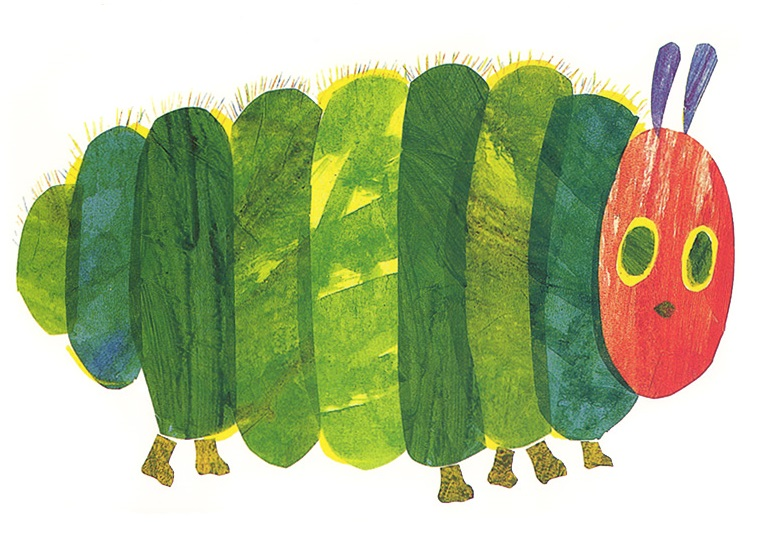
\includegraphics[width=\linewidth]{bilder/caterpillar.jpg}
\caption[Caterpillar]{Caterpillar\cite{caterpillar}}
\label{fig:caterpillar}
\end{wrapfigure}

Lorem ipsum dolor sit amet, consectetur adipiscing elit. Duis blandit, eros vel convallis scelerisque, ante risus hendrerit erat, id luctus urna velit in risus. Nunc nec viverra eros. Duis nisl mi, pharetra non massa ut, scelerisque scelerisque nisi. Donec faucibus nulla id risus condimentum viverra. Aliquam feugiat felis id massa tincidunt, nec malesuada lectus congue. Curabitur sagittis sapien ut augue cursus, eu congue purus sodales. 

Lorem ipsum dolor sit amet, consectetur adipiscing elit. Ut pulvinar viverra mollis. Proin magna justo, congue eget porta ut, maximus vel augue. Donec vehicula leo eu nisi vulputate blandit. Donec ultricies erat in eros suscipit, sit amet mattis elit vulputate. 

\begin{table}[hb]
\scriptsize
\begin{minipage}{0.49\linewidth}
\centering
\begin{tabular}{||c | r | r | r |} 
    \hline
    \textbf{Nr.} & \textbf{\# Ergeb.} & \textbf{PostgreSQL} & \textbf{MongoDB} \\ [0.5ex]
    \hline\hline
    \multirow{3}{*}{1.1} & \multirow{3}{*}{4.678} 
      & 0,9548 s & 0,3056 s \\
    & & 0,8997 s & 0,1290 s \\
    & & 0,9101 s & 0,1213 s \\
    \hline
    \multirow{3}{*}{1.2} & \multirow{3}{*}{4.678} 
      & 1,1088 s & -- \\
    & & 1,2218 s & -- \\
    & & 1,2137 s & -- \\
    \hline
    \multirow{3}{*}{1.3} & \multirow{3}{*}{4.678} 
      & 0,0403 s & -- \\
    & & 0,0412 s & -- \\
    & & 0,0401 s & -- \\
    \hline
    \multirow{3}{*}{2} & \multirow{3}{*}{4.678} 
      & 0,9498 s & 0,1466 s \\
    & & 0,9729 s & 0,1083 s \\
    & & 0,9071 s & 0,1066 s \\
    \hline
    \multirow{3}{*}{3} & \multirow{3}{*}{10.043} 
      & 0,2779 s & 0,3600 s \\
    & & 0,3079 s & 0,2429 s \\
    & & 0,2992 s & 0,2498 s \\
    \hline
    \multirow{3}{*}{4} & \multirow{3}{*}{2} 
      & 0,0018 s & 0,0727 s \\
    & & 0,0009 s & 0,0138 s \\
    & & 0,0009 s & 0,0070 s \\
    \hline
    \multirow{3}{*}{5} & \multirow{3}{*}{253.755}
      & 3,5117 s & 126,0782 s \\
    & & 3,4656 s & 106,1470 s \\
    & & 3,3282 s & 107,9439 s \\
    \hline
\end{tabular}
\end{minipage}
%
\begin{minipage}{0.49\linewidth}
\centering
\begin{tabular}{|c | r | r | r ||} 
    \hline
    \textbf{Nr.} & \textbf{\# Ergeb.} & \textbf{PostgreSQL} & \textbf{MongoDB} \\ [0.5ex] 
    \hline\hline 
    \multirow{3}{*}{6} & \multirow{3}{*}{5.141}
      & 2,1497 s & 12,1915 s \\
    & & 1,8485 s & 11,6134 s \\
    & & 1,7347 s & 11,2647 s \\
    \hline
    \multirow{3}{*}{7} & \multirow{3}{*}{694.907} 
      & 6,3388 s & 23,2439 s \\
    & & 6,6917 s & 22,4676 s \\
    & & 6,6002 s & 22,9043 s \\
    \hline
    \multirow{3}{*}{8} & \multirow{3}{*}{0} 
      & 0,0018 s & 0,0011 s \\
    & & 0,0008 s & 0,0009 s \\
    & & 0,0008 s & 0,0008 s \\
    \hline
    \multirow{3}{*}{9.1} & \multirow{3}{*}{1.635.965} 
      & 27,0328 s & 68,7589 s \\
    & & 28,4229 s & 58,9914 s \\
    & & 27,9176 s & 64,8253 s \\
    \hline
    \multirow{3}{*}{9.2} & \multirow{3}{*}{1.635.965} 
      & 12,2981 s & 73,4722 s \\
    & & 11,5675 s & 63,1674 s \\
    & & 11,4067 s & 68,5112 s \\
    \hline
    \multirow{3}{*}{10.1} & \multirow{3}{*}{14.222.062} 
      & 113,2476 s & 373,5514 s \\
    & & 107,6503 s & 370,8531 s \\
    & & 112,4459 s & 373,4111 s \\
    \hline
    \multirow{3}{*}{10.2} & \multirow{3}{*}{14.222.062} 
      & 143,6760 s & -- \\
    & & 141,0328 s & -- \\
    & & 142,5101 s & -- \\
    \hline
\end{tabular}
\end{minipage}
\caption{Beispieltabelle eines Benchmarks}
\label{tab:benchmark_results}
\end{table}

\chapter{Beispiel eines Code-Kapitels}

\section{Anforderungen}

Hier ein inline-codeblock: \lstinline[language=pseudo]{stop(); // Hammertime!}.\cite{tuoski:2022}

Oder so \lstinline[language=sql]{SELECT * FROM} wie hier.


\paragraphnl{Einfügen}

Aliquam molestie fermentum vestibulum. Cras egestas molestie ipsum, vitae malesuada ante consectetur id. 

\paragraphnl{Löschen}

In turpis neque, pharetra eget neque vel, rhoncus tincidunt ex. Sed lacinia fermentum odio quis faucibus. Phasellus blandit orci vitae ipsum rutrum aliquam. 

\paragraphnl{Ändern}

Fusce ipsum nisl, luctus in interdum non, sodales sed lacus. Fusce vitae fermentum tellus, vitae feugiat magna. 

\section{Implementierung}

Fusce luctus eros sem, id porttitor odio vestibulum sed. Etiam nisl eros, mollis rhoncus dolor vel, consectetur dignissim eros. Donec eu justo et ipsum posuere porttitor vitae quis lacus. 

\begin{wrapfigure}[26]{l}{0.5\linewidth}
% Sprache "sql" ist in header-datei definiert
\begin{lstlisting}[language=sql]
CREATE TABLE IF NOT EXISTS 
"Personen" (
    id serial NOT NULL,
    name text NOT NULL,
    geb_datum date NOT NULL,
    PRIMARY KEY (id)
);

CREATE OR REPLACE FUNCTION 
pruefe_alter()
    RETURNS TRIGGER
    LANGUAGE 'plpgsql'
AS $$
DECLARE
	alter_jahre int;
BEGIN
	SELECT date_part(
	    'year', 
	    age(NEW.geb_datum::TIMESTAMP))
	INTO alter_jahre;
	
	IF alter_jahre < 18 THEN
	    RAISE EXCEPTION 
	        'Person ist nicht volljaehrig';
	END IF;
	
	RETURN NEW;
END;
$$;
	
CREATE OR REPLACE TRIGGER 
trigger_person_einfügen
	BEFORE INSERT ON "Personen"
	FOR EACH ROW
	EXECUTE PROCEDURE pruefe_alter();
\end{lstlisting}
\captionsetup{type=figure}
\captionof{figure}{Beispiel einer\\Trigger-Definition}
\label{fig:trigger_example}
\end{wrapfigure}

Integer venenatis convallis erat, sit amet elementum odio egestas interdum. Phasellus sagittis vestibulum libero vel sodales. Phasellus a facilisis felis, vel mollis velit. Quisque pulvinar turpis vitae bibendum condimentum. Nulla facilisi. Praesent iaculis euismod eros et consequat. Nullam efficitur facilisis sapien. Aenean non laoreet lectus. Phasellus tellus lorem, ullamcorper vel aliquam ut, sollicitudin accumsan nibh. 

Fusce luctus eros sem, id porttitor odio vestibulum sed. Etiam nisl eros, mollis rhoncus dolor vel, consectetur dignissim eros. Donec eu justo et ipsum posuere porttitor vitae quis lacus. Duis convallis tellus non nibh ultrices, eget imperdiet metus iaculis. Integer non feugiat ante. Etiam felis massa, interdum eu egestas vel, eleifend id erat. In nec est ac orci elementum porttitor non non lorem. 

\clearpage

\subsection{Unterthema}

Vivamus quis lacus quis urna suscipit auctor. Nunc dignissim massa eu leo condimentum euismod. 

\subsection{Voraussetzungen}

Nunc mattis quis mauris a pharetra. Duis eu iaculis magna, id tristique dui. Duis sagittis mauris id elit maximus auctor. 

\subsection{Einfügen}

\paragraphnl{Einfügen aus Datei}

Pellentesque vitae ipsum elementum, iaculis enim mollis, fringilla sem. Integer eget odio porta, congue quam 

\subsection{Einfügen aus Webrequest}

Nulla imperdiet turpis in lorem eleifend aliquet sed ac libero. Morbi sed ultricies ipsum. 

\chapter{Zusammenfassung}

\section{Fazit}

Proin gravida dictum faucibus. Sed at semper lectus. Nam ultrices volutpat porta. Nulla non eros sagittis, sodales diam eget, cursus arcu. Integer ipsum metus, convallis a felis in, convallis aliquet urna. Morbi vel odio sed magna aliquam finibus. Proin blandit quis est ac mollis.\cite{join_study}

\section{Ausblick}

Fusce luctus eros sem, id porttitor odio vestibulum sed. Etiam nisl eros, mollis rhoncus dolor vel, consectetur dignissim eros. 

\subsection{Thema\#1}

Integer venenatis convallis erat, sit amet elementum odio egestas interdum. Phasellus sagittis vestibulum libero vel sodales. Phasellus a facilisis felis, vel mollis velit. Quisque pulvinar turpis vitae bibendum condimentum. Nulla facilisi. Praesent iaculis euismod eros et consequat. Nullam efficitur facilisis sapien. Aenean non laoreet lectus. Phasellus tellus lorem, ullamcorper vel aliquam ut, sollicitudin accumsan nibh. 

\subsection{Thema\#2}

Vivamus quis lacus quis urna suscipit auctor. Nunc dignissim massa eu leo condimentum euismod. Nunc mattis quis mauris a pharetra. Duis eu iaculis magna, id tristique dui. Duis sagittis mauris id elit maximus auctor. Pellentesque vitae ipsum elementum, iaculis enim mollis, fringilla sem. 


\appendix
\chapter{Anhang}

\vspace{-1cm}
\section{Unterteilung der Annotations-Attribute}
\label{sec:attribute_grouping}

\vspace{-1cm}
\begin{minipage}[t]{0.47\linewidth}
\begin{lstlisting}[language=json,title=Face Position Orientation]
{
    "bounding_box": {
        "position": {
            "x": int,
            "y": int
        }
        "width": int,
        "height": int
    },
    "eyes": {
        "left": {
            "x": int,
            "y": int
        },
        "right": {
            "x": int,
            "y": int
        }
    },
    "orientation": {
        "yaw": int,
        "pitch": int,
        "roll": int
    },
    "is_gaze_frontal": bool,
    "is_pose_ok": bool
}
\end{lstlisting}
\end{minipage}
%
\hspace{0.01\linewidth}
%
\begin{minipage}[t]{0.47\linewidth}
%
\begin{minipage}[t]{\linewidth}
\begin{lstlisting}[language=json,title=Image Details]
{
    "is_color_ok": bool,
    "is_exposure_ok": bool,
    "is_focus_ok": bool,
    "is_occluded": bool,
    "has_hotspots": bool,
    "has_shadows": bool,
    "has_red_eyes": bool
}
\end{lstlisting}
\end{minipage}
%
\begin{minipage}[t]{\linewidth}
\begin{lstlisting}[language=json,title=Face Demographics]
{
    "age": int,
    "age_estimated": int,
    "ethnicity": int,
    "gender": string
}
\end{lstlisting}
\end{minipage}
%
\begin{minipage}[t]{\linewidth}
\begin{lstlisting}[language=json,title=Face Details]
{
    "is_disguised": bool,
    "is_expression_neutral": bool,
    "eyes_open": bool,
    "has_facial_hair": bool,
    "mouth_closed": bool,
    "has_glasses": bool,
    "has_glasses_reflection": bool,
    "no_face_found": bool,
}
\end{lstlisting}
\end{minipage}
%
\end{minipage}

\clearpage

\begin{minipage}[t]{\linewidth}
\begin{lstlisting}[language=python,title=AnnotationSchema.py,firstnumber=34]
class AnnotationBase(BaseModel):
    age: StrictInt = None
    age_estimated: StrictInt = None
    gender: Gender = None
    ethnicity: StrictInt = None
    bounding_box: BoundingBox = None
    orientation: Orientation = None
    eyes: Eyes = None
    eyes_open: bool = None
    mouth_closed: bool = None
    is_disguised: bool = None
    is_expression_neutral: bool = None
    is_gaze_frontal: bool = None
    is_pose_ok: bool = None
    is_color_ok: bool = None
    is_exposure_ok: bool = None
    is_background_ok: bool = None
    is_focus_ok: bool = None
    is_occluded: bool = None
    has_hotspots: bool = None
    has_shadows: bool = None
    has_glasses: bool = None
    has_facial_hair: bool = None
    has_glasses_reflection: bool = None
    has_red_eyes: bool = None
    no_face_found: bool = None


class AnnotationAllowExtra(AnnotationBase, extra=Extra.allow):
    pass


class AnnotationForbidExtra(AnnotationBase, extra=Extra.forbid):
    pass
\end{lstlisting}
\end{minipage}

\end{onehalfspace}

%%%%%%%%%%%%%%%%%%%%%%%%%%%%%%%%%%%%%%%%%%%%%%%%%%%%%%%%%%%%%%%%%%%

\printbibliography{} % create with BibTeX

\chapter*{Eidesstattliche Erklärung}
\addcontentsline{toc}{chapter}{Eidesstattliche Erklärung}

Ich erkl\"are hiermit an Eides statt, dass ich die vorliegende Arbeit selbstst\"andig und ohne Benutzung anderer als der angegebenen Hilfsmittel angefertigt habe; die aus fremden Quellen direkt oder indirekt \"ubernommenen Gedanken sind als solche kenntlich gemacht. Die Arbeit wurde bisher in \"ahnlicher Form keiner anderen Pr\"ufungskommission vorgelegt und auch nicht ver\"offentlicht.

\bigskip
\bigskip
\bigskip
\bigskip
	
\begin{multicols}{2}
  \raggedright
  Ort, Datum
    
  \raggedleft
  \authorname
  
\end{multicols}


\end{document}
